
% TODO: not relevant here, move to introduction
%Agricultural technologies have been a source of innovation since the dawn of humanity. The quest for more efficient food
%production has driven significant research, and above all, automation stands out as a paramount achievement in the
%modern world. A great tool to improve the automation process is \gls{IoT}, a concept that refers to the interconnection
%of physical devices in a diffused network; each device collects valuable and localized information that is used to
%improve efficiency, productivity, and decision making.\\

The goal of this chapter is to describe the intended use case scenario for Bacco and to provide a brief
introduction to the \gls{LoRaWAN} protocol with a focus on the mentioned scenario.

\section{IoT For Agriculture}

\subsection{Benefits}
The refinment of automation systems used in agriculture has been a costant interest throughout all history of
industry due to the huge positive impact it has brought to society. If \gls{IoT} is introduced
in agricultural contexts, it could bring lots of benefits:
\begin{itemize}
    \item Precision farming: IoT devices enable farmers to collect real-time data on environmental variables. This data
        helps optimize irrigation, fertilization, and pest control, leading to higher crop yields and reduced resource
        waste;
    \item Decision making: the generated data provides farmers with insights into crop health, growth
        patterns, and yield predictions. This allows them to make informed decisions regarding planting, harvesting, and
        resource allocation, resulting in better outcomes;
    \item Remote monitoring and management: farmers can remotely monitor their fields through IoT devices,
        reducing the need for constant physical presence. This is especially valuable for managing large or distant farms;
    \item Automation and labor savings: automation can handle tasks such as planting, irrigation, and
        harvesting. This not only reduces labor costs but also frees up farmers to focus on more strategic aspects of
        their operations;
    \item Knowledge sharing and collaboration: IoT platforms can facilitate the exchange of best practices, data, and
        insights among farmers, researchers, and agricultural experts, promoting knowledge sharing;
    \item Sustainability and environmental impact: trough optimized resource use, IoT contributes to more sustainable
        and environmentally friendly agricultural practices;
\end{itemize}

\subsection{Requirements}
Where \gls{IoT} is applied to agriculture, a set of unique and challenging requirements come into play:
\begin{itemize}
    \item Power management: many remote agricultural locations lack a reliable power source. Devices need to be
        designed with energy-efficient technology paired with high-energy batteries and/or alternative power sources like solar
        panels to ensure uninterrupted operation;
    \item Connectivity and coverage: many agricultural areas lack reliable internet connectivity, which can hinder
        transmissions between IoT devices and central systems. Even by using alternative solutions such as \glspl{LPWAN}
        like LoRaWAN or Bacco, long distances and physical barriers are problems that need to be faced;
    \item Reliability and fail-safeness: human operation is not always convenient or even possible in
        some cases, so having a fail-safe system is crucial to have maintain functionality;
    \item Physical damage: constant exposure to weather conditions undermines the integrity of the devices used in the
        open field, so it is important to use of materials that are resistant to such circumstances;
    \item Environmental impact: some ecosystems may be influenced by the introduction of alien objects or
        electromagnetic radiation;
    \item Cost: initial setup costs for devices, sensors, and infrastructure can be high, which may discourage small
        farmers from adopting these technologies;
    \item Regulations and compliance: different regions may have varying regulations concerning the elecromagnetic
        specturm usage, environmental monitoring, and technology deployment. Adhering to these regulations can be complex when
        implementing solutions across different areas;
    \item User-friendly interfaces: the user interfaces need to be intuitive, especially for farmers who might not
        have extensive technical knowledge.
\end{itemize}
This thesis will not comprehensively cover all the aspects mentioned above. Instead, it will just concentrate on the
communication protocol utilized by the network. While all efforts have been directed towards meeting the requirements,
it is important to note that mechanical, environmental, economic, and legal considerations will be left to future
discussions.

\section{An Already Available Technology: LoRaWAN}
One of the most promising technologies in \gls{IoT} for agrigulture is \gls{LoRaWAN}, an open protocol built on top of
Semtech's proprietary LoRa modulation. It provides all the necessary software components to build a suitable network
that is reliable, power efficient and scalable according to extensive past research. See \cite{lorawan_agriculture_1}
and \cite{lorawan_agriculture_2} for reference.\\
A LoRaWAN network consists of sender nodes and gateways. When a sender node broadcasts a LoRa transmission, it can be
received by one or more gateways, that can store the information or forward it to a web server through the Internet.
This kind of message is called uplink. Gateways might need to transmit data to the sender nodes, this kind message is
called downlink. Gateways can be self-owned with a custom configuration or can be part of an existing community such as
\gls{TTN} or Helium.\\
Senders can uplink at any time because gateways are always listening to transmissions. On the other hand, downlink
messages need to be scheduled as it is not always possible for a sender node to be listening continuously because of
the limited power budget. To achieve that, LoRaWAN defines 3 classes of devices called class A, class B and class C.
The classes are sorted by increasing energy demand, so class A stands out in agricultural
contexts thanks to its superior power efficiency when compared to classes B and C. In this mode, a downlink message can
only be sent in 2 time slots at pre-defined delays subsequently to the reception of an uplink message. Figure \ref{img:
lorawan class a} shows a schematic version of the time slot management.

\begin{figure}[ht]
    \centering
    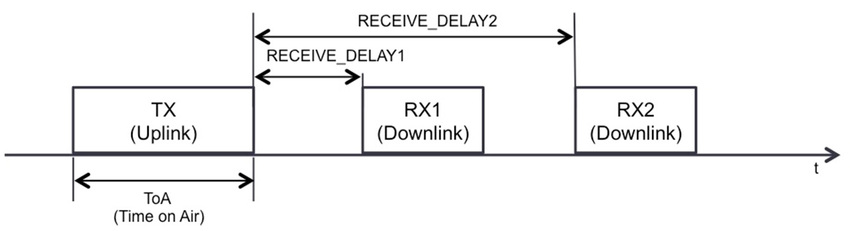
\includegraphics[width=\linewidth]{images/lorawan_class_a.png}
    \caption{LoRaWAN class A device operation.}
    \label{img: lorawan class a}
\end{figure}

\section{Real Word Use Case: Small Vineyard}
I will now describe a real world scenario in which \gls{IoT} can be integrated to 

\subsection{LoRaWAN Setup Using A Public Gateway}
%TODO: point out unnecessary things that LoRaWAN does
To build a functional network, it is sufficent


\subsection{LoRaWAN Setup Using An Owned Gateway}
%TODO: point out unnecessary things that LoRaWAN does

\subsection{Proposed Bacco Setup}
- What can be cut off?
- Could an equivalent system exist with a lower cost and power consumption?

